(Gusfield Chapter 2)

\newthought{Key Ideas} of the Boyer-Moore algorithm: right-to-left scan, bad character rule, good suffix rule.

\section{Bad Character Rule}

The intuition behind the bad character rule is as follows. Suppose we have the pattern $P$ and text $T$, and the rightmost character of $P$ is aligned to the character $x$ in $T$, where $x \neq y$. If we know the position of the rightmost $x$ in $P$, we can safely shift $P$ by that amount to the right so that the $x$ in $P$ aligns with the $x$ in $T$. Furthermore, if we know that $x$ is not in $P$, we can shift $P$ completely past the $x$ in $T$. This intuition is formalized below, as shown in Gusfield's book.

\begin{definition}
    For each character $x$ in the alphabet, let $R(x)$ be the position of the rightmost occurrence of character $x$ in $P$. If $x$ does not occur in $P$, $R(x) = 0$.
\end{definition}

\begin{rules}[Bad Character Rule] \index{bad character rule}
    \normalfont
    Suppose for a particular alignment of $P$ against $T$, the rightmost $n-i$ characters of $P$ match their counterparts in $T$, but the next character to the left $P(i)$ mismatches with its counterpart in $T$, say at position $k$ in $T$. The \textit{\textbf{bad character rule}} says that $P$ should be shifted right by $\max\{1,\, i-R(T(k))\}$ places. That is, if the rightmost occurrence of $T(k)$ in $P$ is in position $j < i$, then shift $P$ so that the $j$th character of $P$ is matched to the $k$th character of $T$ (or completely shifting $P$ past $k$th position if the $k$th character of $T$ does not occurr in $P$). Otherwise, if $j > i$, shift $P$ by one position.
\end{rules}

\section{Extended Bad Character Rule}

Note that the bad character rule allows us to shift more than one character only when the mismatched character show up at a position left of the mismatched point. However, it is not as helpful if the character only occurs in $P$ on the right side of the mismatched point. The \textit{\textbf{extended bad character rule}} addresses this issue.

\begin{rules}[Extended Bad Character Rule] \index{extended bad character rule}
    \normalfont
    When a mismatch occurs at position $i$ of $P$ and the mismatched character in $T$ is $x$, then shift $P$ to the right so that the closest $x$ to the left position $i$ in $P$ is matched with the $x$ in $T$.
\end{rules}

\begin{figure}[htbp]
    \centering
    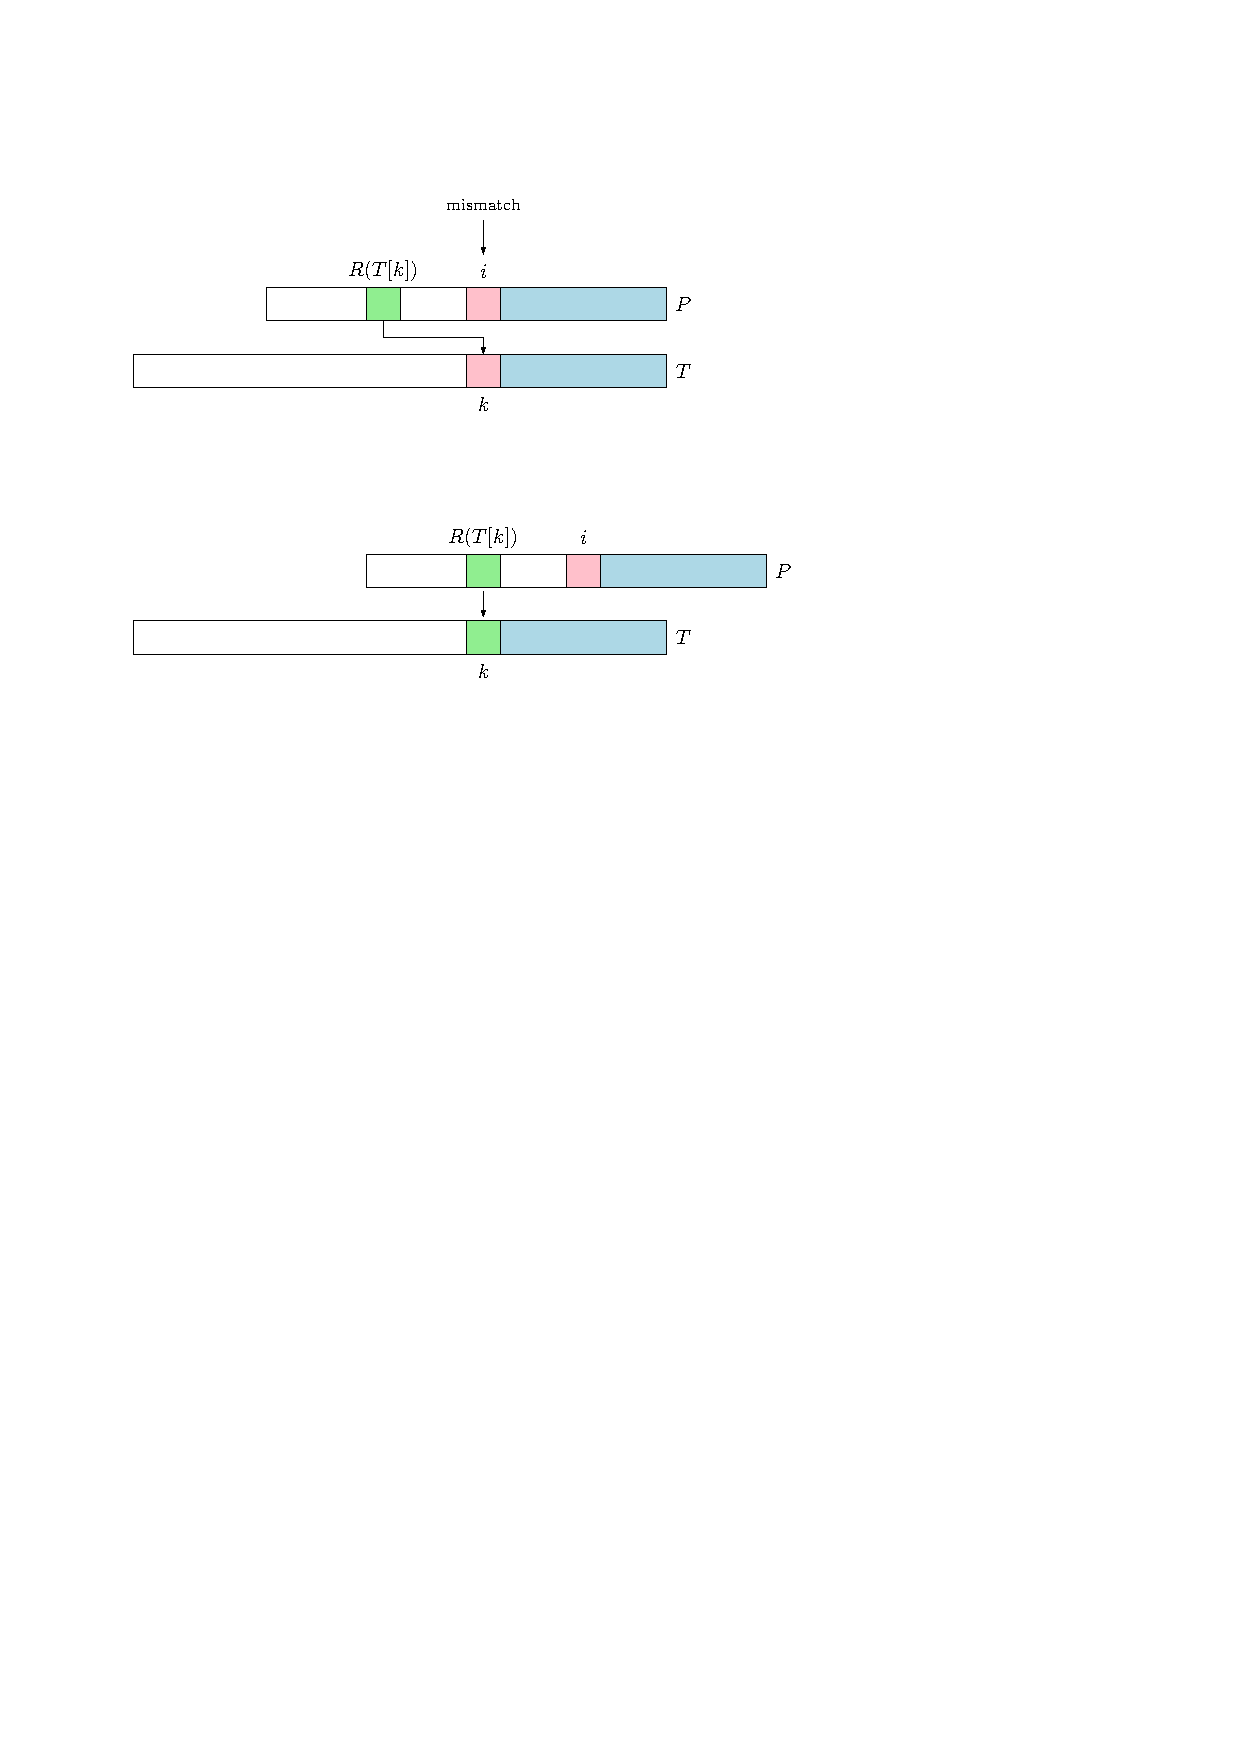
\includegraphics[width=0.8\linewidth]{boyer-moore/bad-character-rule.pdf}
    \caption{The bad character rule says to shift as much as possible so that a mismatch becomes a match.}
    \label{fig:boyer-moore-bad-char-rule}
\end{figure}

\subsection{Preprocessing for Bad Character Rule}

The bad character rule is quite straightforward to implement. In the preprocessing for the bad character rule, we find, for each position $i$ in the pattern $P$ and for each characther $x \in \Sigma$, the position of the closest occurrence of $x$ in $P$ to the left of $i$. This uses an $n \time \Sigma$ matrix. However, the time complexity for building this lookup table and the space required for it could be massive, depending on the length of the pattern and the size of the alphabet. It is also not hard to see that this approach can be quite space inefficient and we can end up store duplicate information over and over.

\begin{marginfigure}
    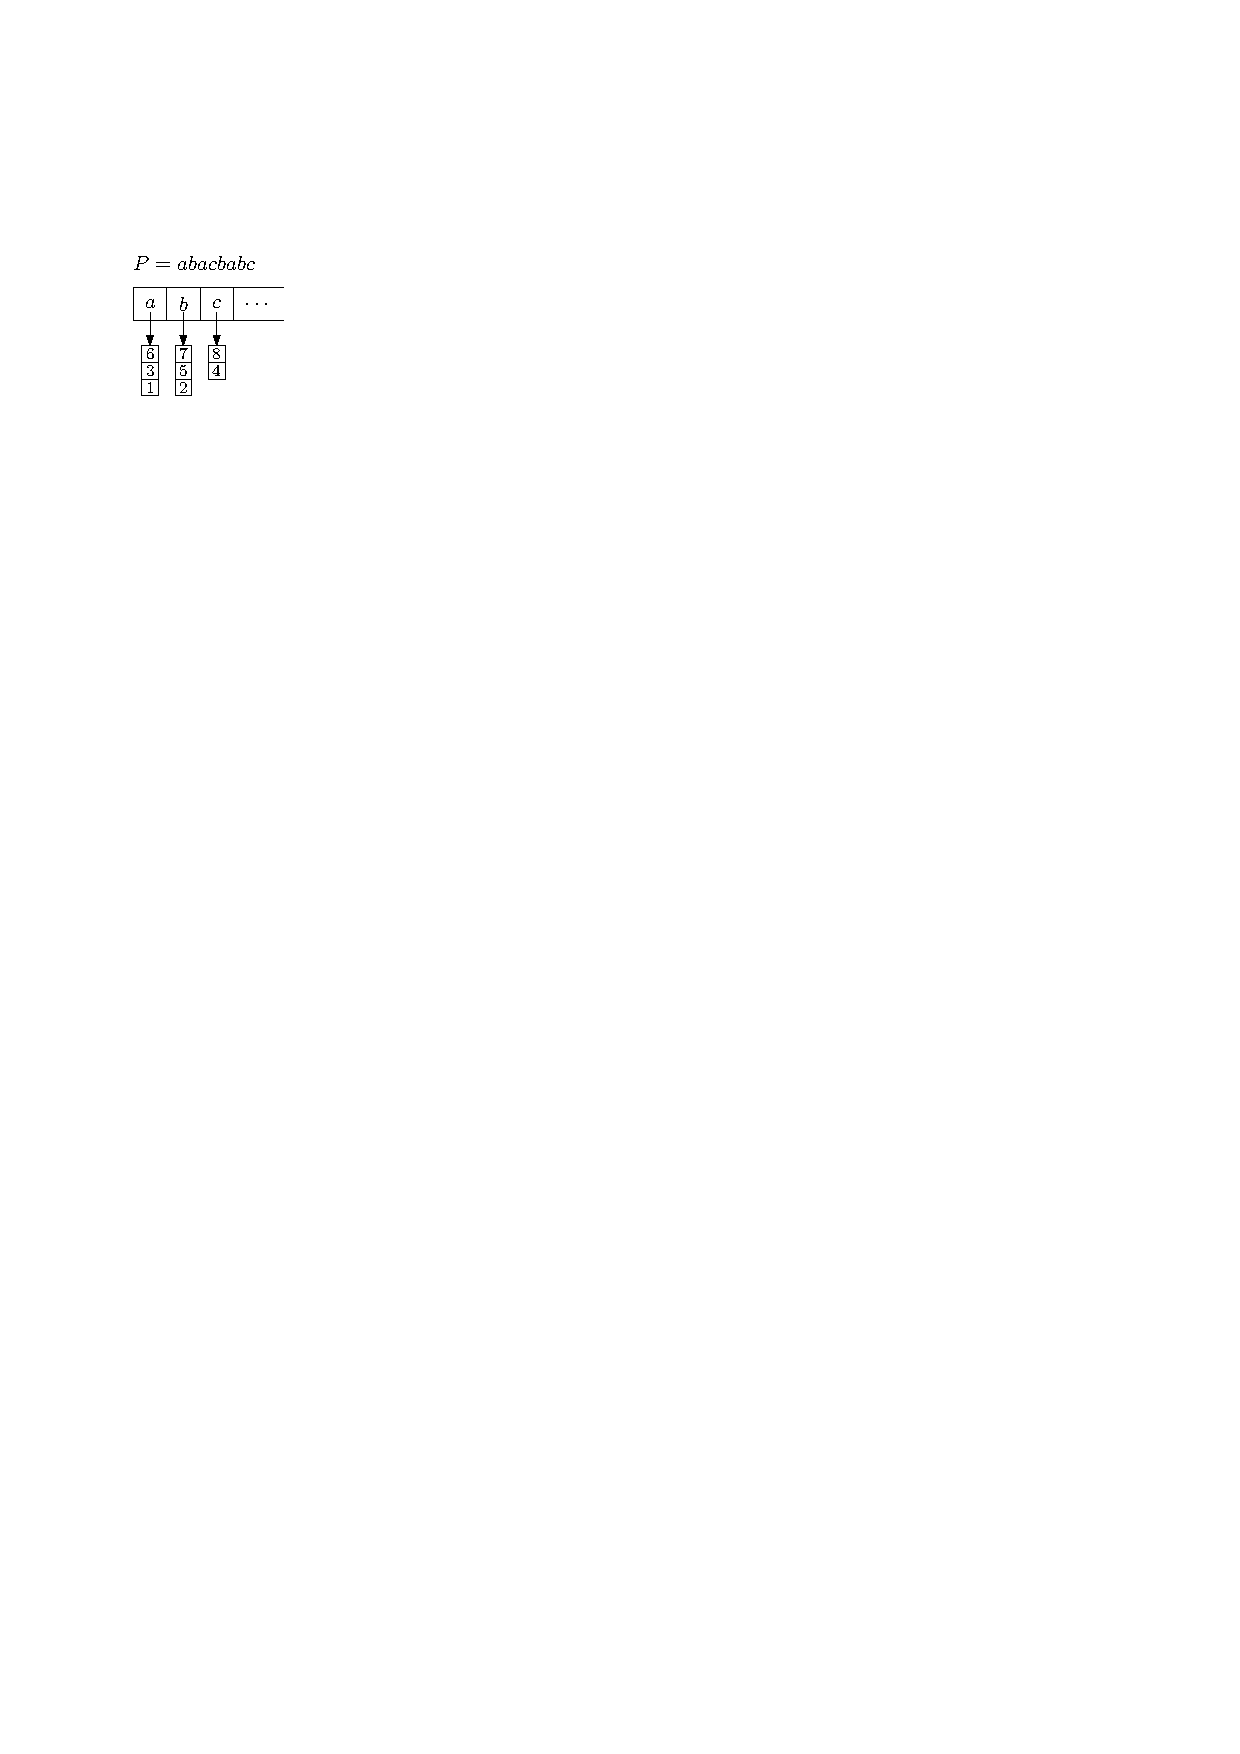
\includegraphics[width=0.5\linewidth]{boyer-moore/bad-character-rule-table.pdf}

    \hfill
    
    \caption{Table for storing information obtained from the bad character rule preprocessing.}
    \label{fig:bad-character-rule-table}
\end{marginfigure}

Alternatively, we can scan $P$ from right to left, and for each character $x \in \Sigma$, we keep a list of positions where $x$ occurs in $P$ (think hash table with chaining but just using another array instead of linked list). Since we scan $P$ from right to left, the indices will be stored in decreasing order for each character. It takes $O(n)$ space. During the actual execution of the Boyer-Moore algorithm, we can query this table whenever we need to find the rightmost occurrence of character $x$ left of index $i$. We can use \textit{binary search} for this.

If the alphabet $\Sigma$ is sparse, we can condense it by simply creating a mapping $f$ from $\Sigma \to \N$. The two approaches can be implemented as follows, respectively.

\begin{multicols}{2}
    \begin{codebox}
        \Procname{$\proc{Create-Bad-Char-Table}(P, f)$}
        \li $\id{table} = [\,]$
        \li $\id{row} = [0,\ldots,0]$
        \li \For $i = 1$ \To $|P|$ \Do
            \li $c = P[i]$
            \li $\id{table}.\proc{Append}(\id{row})$
            \li $\id{row}[f(c)] = i + 1$
        \End
        \li \Return $\id{table}$ 
    \end{codebox}
    
    \begin{codebox}
        \Procname{$\proc{Create-Bad-Char-Table}(P, f)$}
        \li $\id{table} = [\,]$
        \li \For $i = |P|$ \textbf{downto} $1$ \Do
            \li $c = P[i]$
            \li $\id{table}[f(c)].\proc{Append}(i)$
        \End
        \li \Return $\id{table}$ 
    \end{codebox}
    
\end{multicols}


\section{Good Suffix Rule}

\begin{rules}[Good Suffix Rule] \index{good suffix rule}
    \normalfont
    Given an alignment of $P$ against $T$, suppose a substring $t$ of $T$ matches a \textbf{suffix} of $P$, but a mismatch occurs at the next comparison to the left. Then, find, if exsits, the right-most copy $t'$ of $t$ in $P$ such that $t'$ is not a suffix of $P$. Shift $P$ to the right so that $t'$ in $P$ is matched with $t$ in $T$.
\end{rules}

Essentially, the \textit{\textbf{good suffix rule}} says we can shift as much as possible such that an \textit{existing match does not become a mismatch}. 

This rule is the weaker version of the good suffix rule used by Boyer and Moore's original publication. We now present a stronger version of the good suffix rule that allows us to prove properties of the Boyer-Moore algorithm more easily.

\section{Strong Good Suffix Rule}

\begin{rules}[Strong Good Suffix Rule] \index{strong good suffix rule}
    \normalfont
    Given an alignment of $P$ against $T$, suppose a substring $t$ of $T$ matches a \textbf{suffix} of $P$, but a mismatch occurs at the next comparison to the left. Then, find, if exsits, the right-most copy $t'$ of $t$ in $P$ such that $t'$ is not a suffix of $P$. Additionally, \textbf{we requires that the character left of $t'$ in $P$ differs from the character to the left of $t$ in $P$}. Shift $P$ to the right so that $t'$ in $P$ is matched with $t$ in $T$.
\end{rules}

\begin{figure}[htbp]
    \centering
    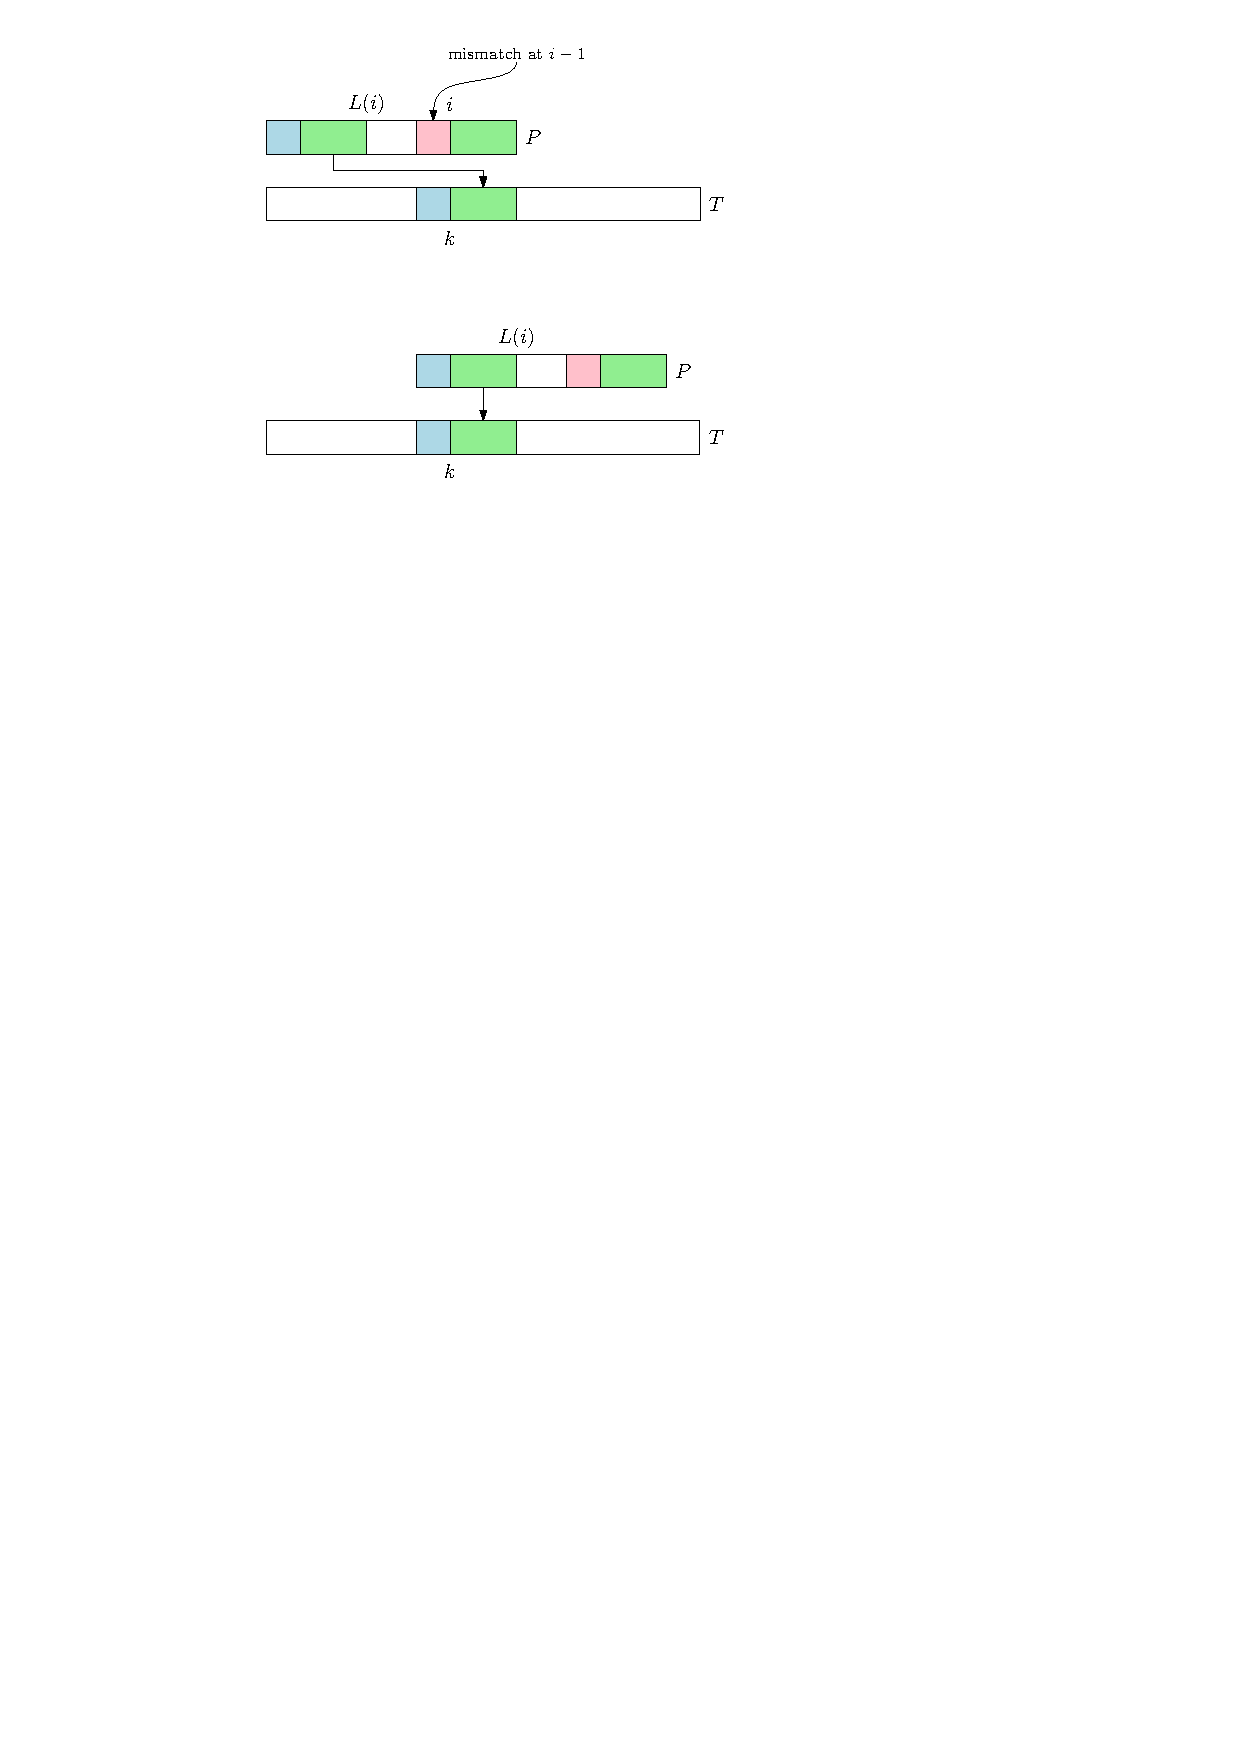
\includegraphics[width=0.6\linewidth]{boyer-moore/good-suffix-rule.pdf}
    \caption{The good suffix rule says we can shift as much as possible so long as a match does not become a mismatch. The additional requirement in the strong good suffix rule ensures that we don't encounter the same mismatch at $P[i-1]$.}
    \label{fig:boyer-moore-good-suffix-rule}
\end{figure}

Note the additional requirement stated in the second-to-last sentence. The addition of this requirement ensures that we don't get the same mismatch. A copy of $t$ is not worth looking at if it results in the same mismatch at the next character to the left. We call this rule the \textit{\textbf{strong good suffix rule}}. It should be obvious that it is safe to shift using the strong good suffix rule. That is, we won't miss any matches if we shift $P$ using the strong good suffix rule. We formalize this idea of correctness in the following theorem.

\begin{theorem}
    The strong good suffix rule does not shift $P$ past an occurrence in $T$.
\end{theorem}

\begin{proof}
    By contradiction. See Gusfield Theorem 2.2.1.
\end{proof}

\subsection{Preprocessing for Good Suffix Rule}


\begin{definition}
    For each $i$, let $L(i)$ be the \textbf{largest position} less than $n$ such that string $P[i\ldots n]$ matches a suffix of $P[1\ldots L(i)]$. If no such position exists, $L(i) = 0$.
    \begin{marginfigure}
        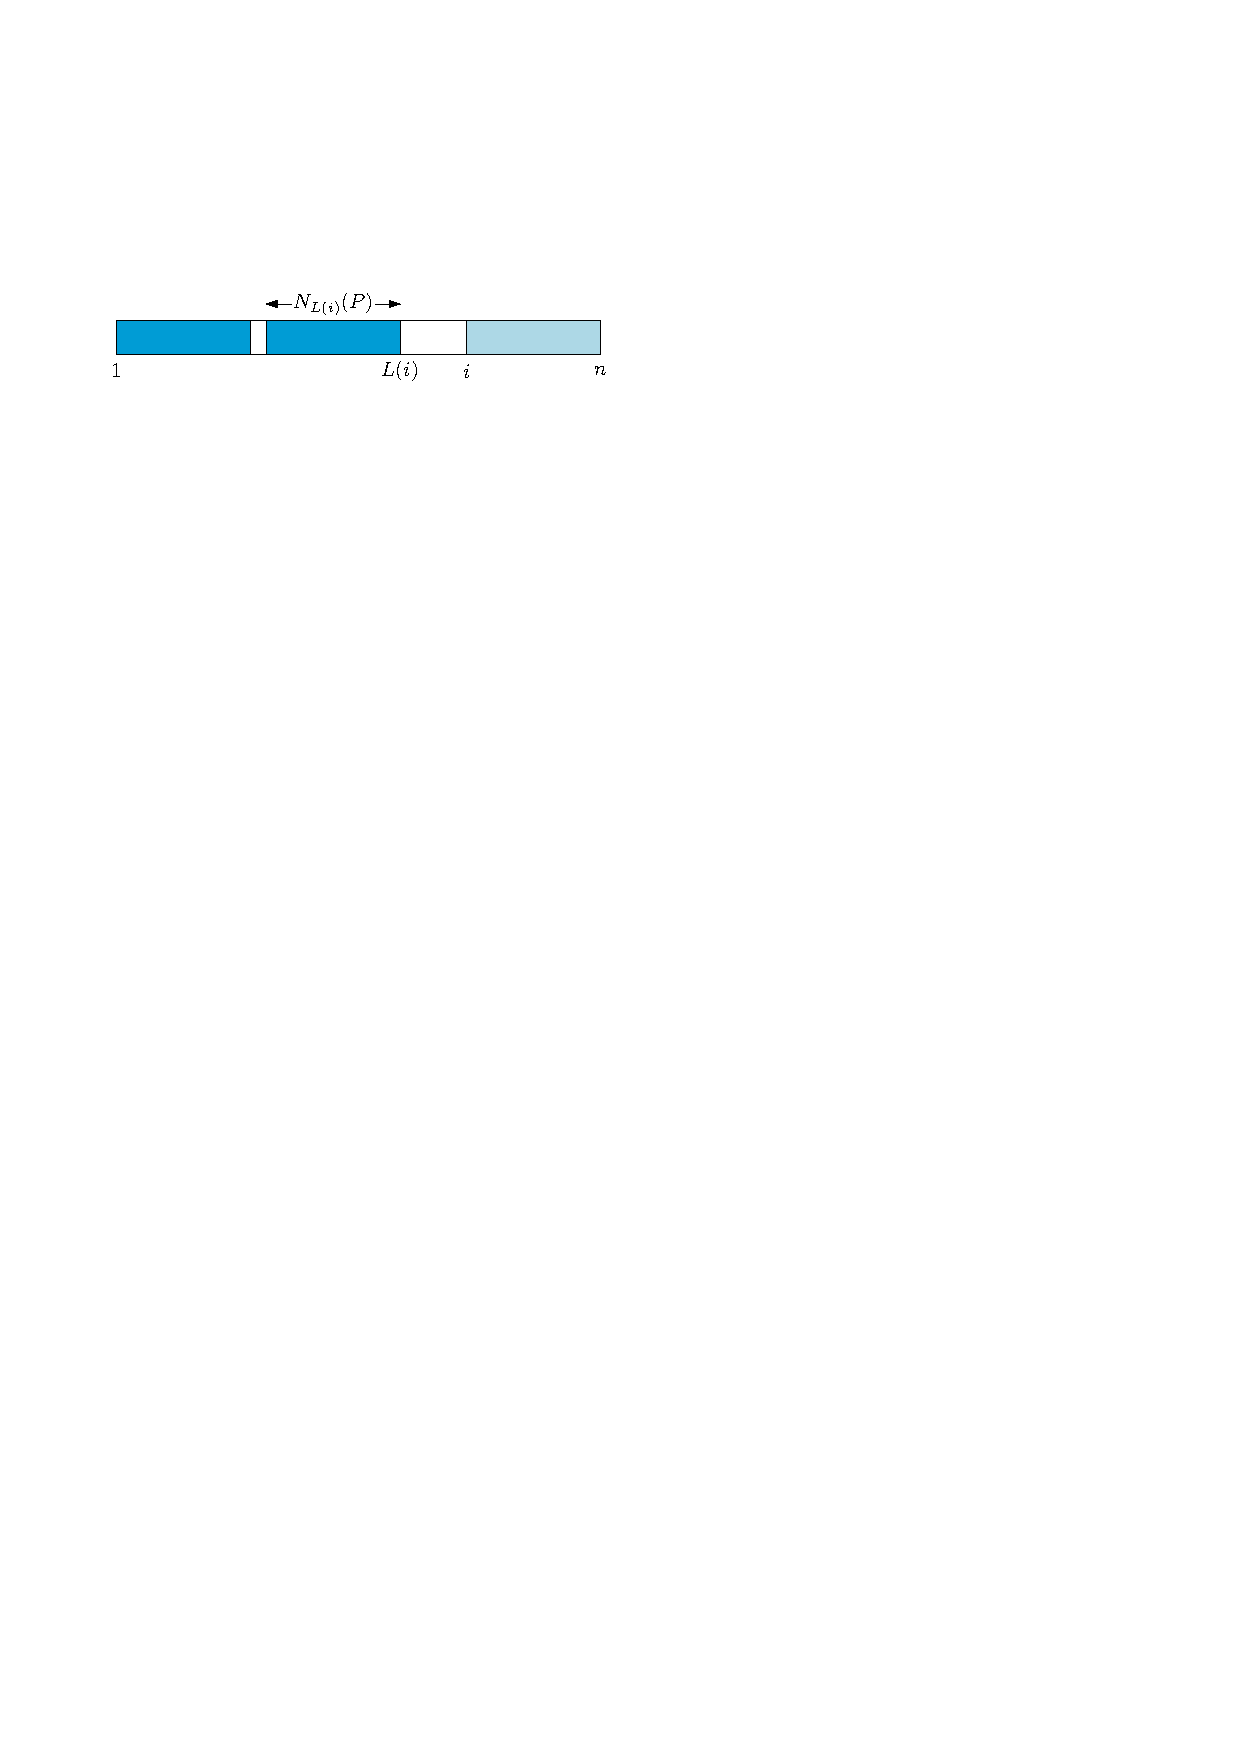
\includegraphics[width=\linewidth]{boyer-moore/good-suffix-Li.pdf}
        \caption{$L(i)$ gives the right-most copy of $t$ that is not a suffix of the whole string.}
        \label{fig:good-suffix-Li}
    \end{marginfigure}
    For each $i$, let $L'(i)$ be the largest position less than $n$ such that string $P[i \ldots n]$ matches a suffix of $P[1\ldots L'(i)]$ and such that the character preceding that suffix is not equal to $P[i-1]$. If no such position exists, $L'(i) = 0$.
\end{definition}

By definition, $L'(i)$ gives the right endpoint of the rightmost copy of $P[i\ldots n]$ that is not a suffix of $P$, and whose preceding character does not equal to $P[i-1]$.

\begin{definition}
    For string $P$, $N_j(P)$ is the length of the \textit{\textbf{longest suffix}} of the substring $P[1\ldots j]$ that is also a \textit{\textbf{suffix}} of the whole string $P$.
\end{definition}

\begin{theorem} \label{thm:good-suffix-Li-property}
    $L(i)$ is the largest index $j$ less than $n$ such that $N_j(P) \geq |P[i\ldots n]|$.
\end{theorem}

\begin{proof}
    By definition of $L$, $L(i)$ is the largest index less than $n$ such that $P[i\ldots n]$ matches a suffix of $P[1\ldots L(i)]$. 
    
    Let $j = L(i)$ in the definition of $N_j$. Then, $N_j(P)$ is the length of the longest suffix of the substring $P[1\ldots L(i)]$ that is also a suffix of the whole string. A suffix of the whole string must also be a suffix of $P[i\ldots n]$. Then, clearly, $N_j(P) \geq |P[i \ldots n]|$ because the substring $P[L(i)-N_j(P)+1 \ldots L(i)]$ can possibly match more characters left of $P[i]$.
\end{proof}

\begin{corollary}
    $L'(i)$ is the largest index $j$ less than $n$ such that $N_i(P) = |P[i\ldots n]| = n-i+1$.
\end{corollary}

\begin{proof}
    Immediate from Theorem \ref{thm:good-suffix-Li-property}. The definition requires that the characters left of $P[i]$ must not be contained in the suffix ending at $L'(i)$.
\end{proof}

One crucial observation is that $N_j$ is, in fact, the exact reverse of $Z_i$ when we talked about the Z-algorithm. Hence, $N_j(P)$ can be computed in linear time for all $j$ in linear time by calling \proc{Compute-Z} on $P^R$ (the reversal of $P$).

\begin{codebox}
    \Procname{$\proc{Compute-L'}(P)$}
    \li $N = \proc{Compute-Z}(P^R)$
    \li \For $i=1$ \To $|P|$ \Do
        \li $L'[i] = 0$ 
    \End
    \li \For $j = 1$ \To $|P|-1$ \Do
        \li $i = n - N[j] + 1$ 
        \li $L'[i] = j$ 
    \End
    \li \Return $L'$ 
\end{codebox}

\begin{definition}
    For string $P$, $l'(i)$ is the length of the \textit{\textbf{longest suffix}} of $P[i\ldots n]$ that is also a \textit{\textbf{prefix}} of the whole string $P$. If none exists, $l'(i)=0$.
    \begin{marginfigure}
        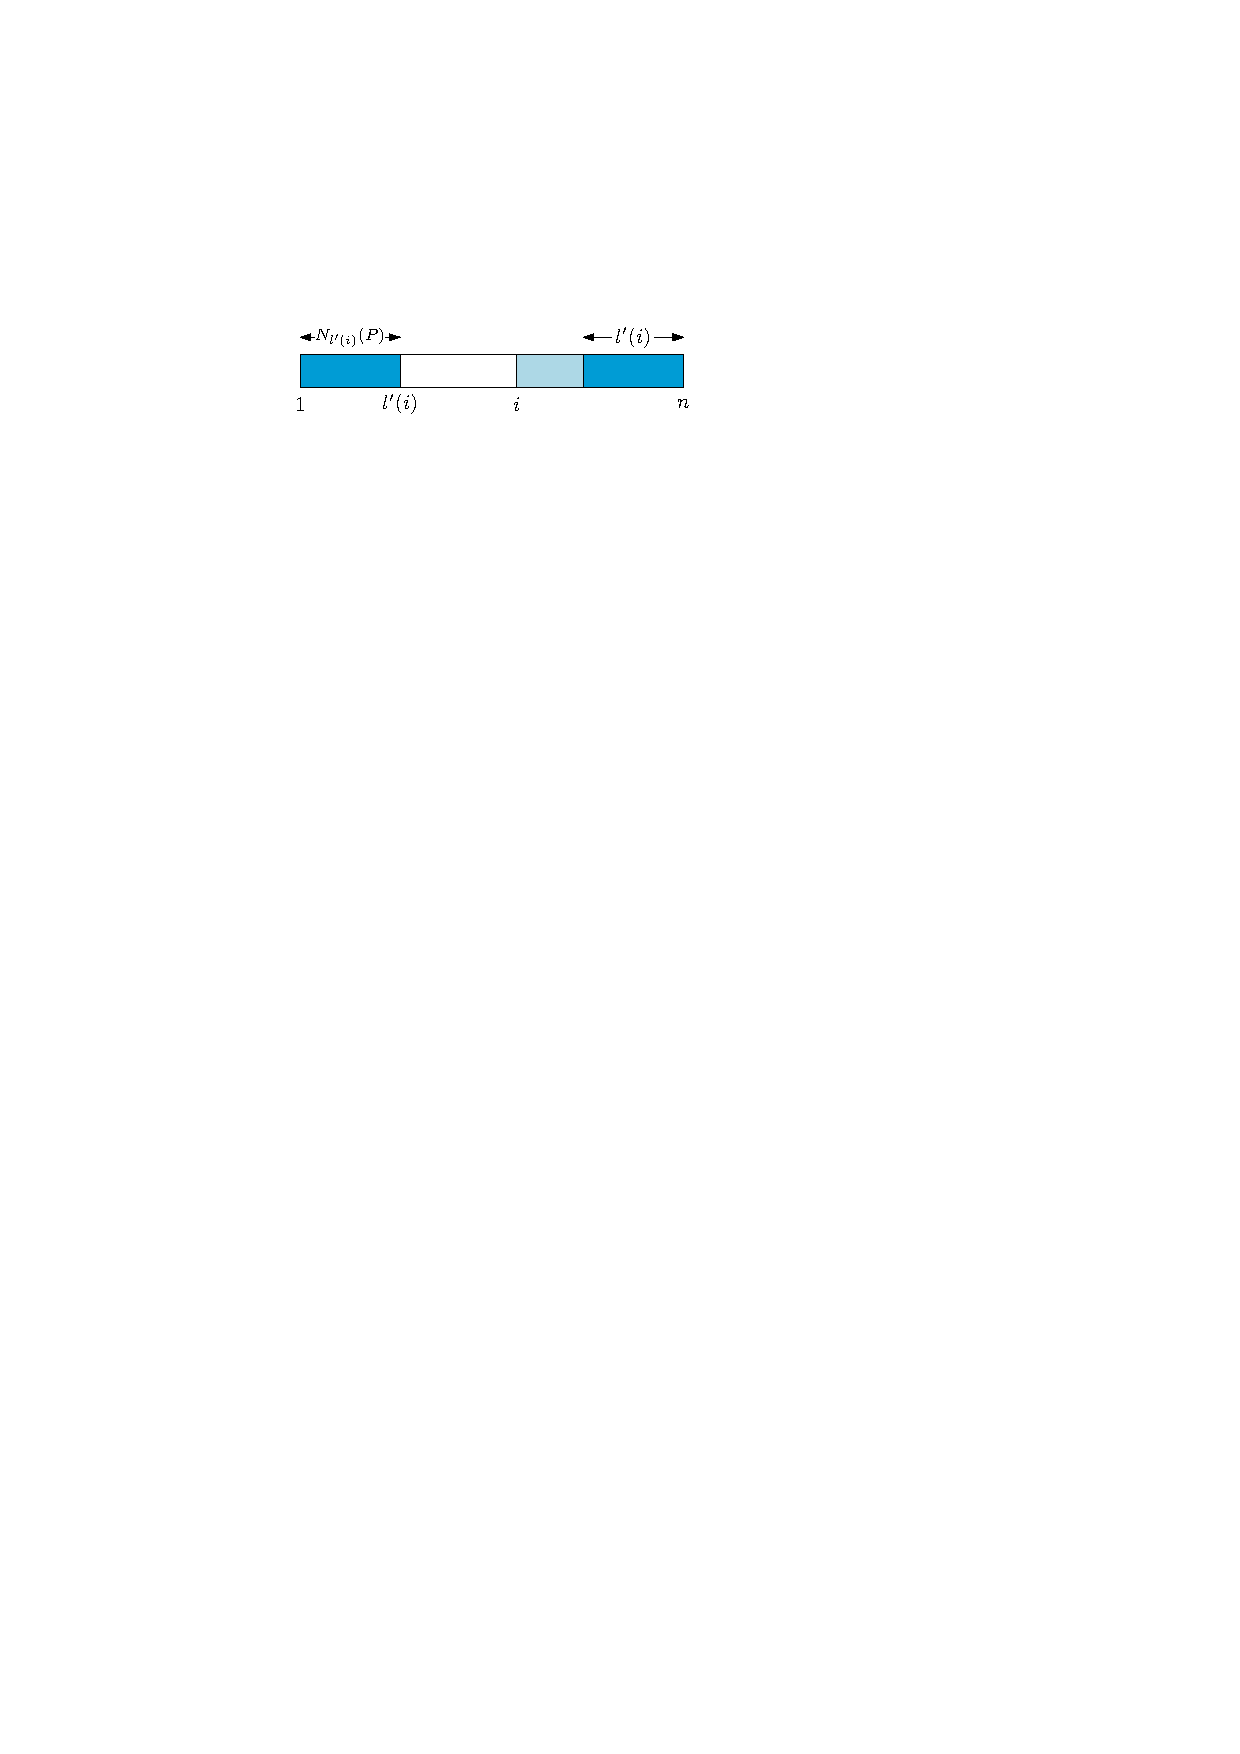
\includegraphics[width=\linewidth]{boyer-moore/good-suffix-ell-i.pdf}
        \caption{$l'(i)$ gives the index of the end of the longest prefix that matches a suffix of $P[i\ldots n]$.}
        \label{fig:good-suffix-ell-i}
    \end{marginfigure}
\end{definition}

\begin{theorem} \label{thm:good-suffix-ell-i-property}
    $l'(i)$ is the largest index $j \leq |P[i\ldots n]| = n-i+1$ such that $N_j(P)=j$.
\end{theorem}

\begin{proof}
    By definition of $l'$, the prefix $P[1\ldots l'(i)]$ is the longest prefix that matches a suffix of $P[i\ldots n]$. So $l'(i) \leq |P[i\ldots n]|$. A suffix of $P[i\ldots n]$ is also a suffix of $P$, so $P[1\ldots l'(i)]$ also matches a suffix of $P$.

    Let $j=l'(i)$ in the definition of $N_j$. Then, by definition of $N_j$, $P[l'(i)-N_{l'(i)}(P)+1\ldots l'(i)]$ is the longest suffix of $P[1\ldots l'(i)]$ that matches a suffix of $P$. The longest suffix of $P[1\ldots l'(i)]$ is $P[1\ldots l'(i)]$ itself, and indeed $P[1\ldots l'(i)]$ matches a suffix of $P$. Hence, $l'(i) = N_{l'(i)}(P)$. The maximality follows from the definition of $l'(i)$.
\end{proof}

\begin{codebox}
    \Procname{$\proc{Compute-$\ell'$}(P)$}
    \li $N = \proc{Compute-Z}(P^R)$
    \li \Comment{initialize $l'$ array}
    \li \For $i = 1$ \To $|P|$ \Do
        \li $l'[i] = 0$
    \End
    \li \Comment{set entires of $l'$ based on Theorem \ref{thm:good-suffix-ell-i-property}}
    \li \For $j = 1$ \To $|P|$ \Do
        \li \If $N[j] \isequal j$ \Then
            \li $l'[|P|-j+1] = j$
        \End
    \End
    \li \Comment{fill in $l'$ for $i$'s left of the longest suffix that matches a prefix}
    \li \For $i = |P|-1$ \textbf{downto} 1 \Do
        \li \If $l'[i] \isequal 0$ \Then
            \li $l'[i] = l'[i+1]$
        \End
    \End
    \li \Return $l'$ 
\end{codebox}

It may not be clear at first what the last for-loop on line 10-12 does. 
\begin{marginfigure}
    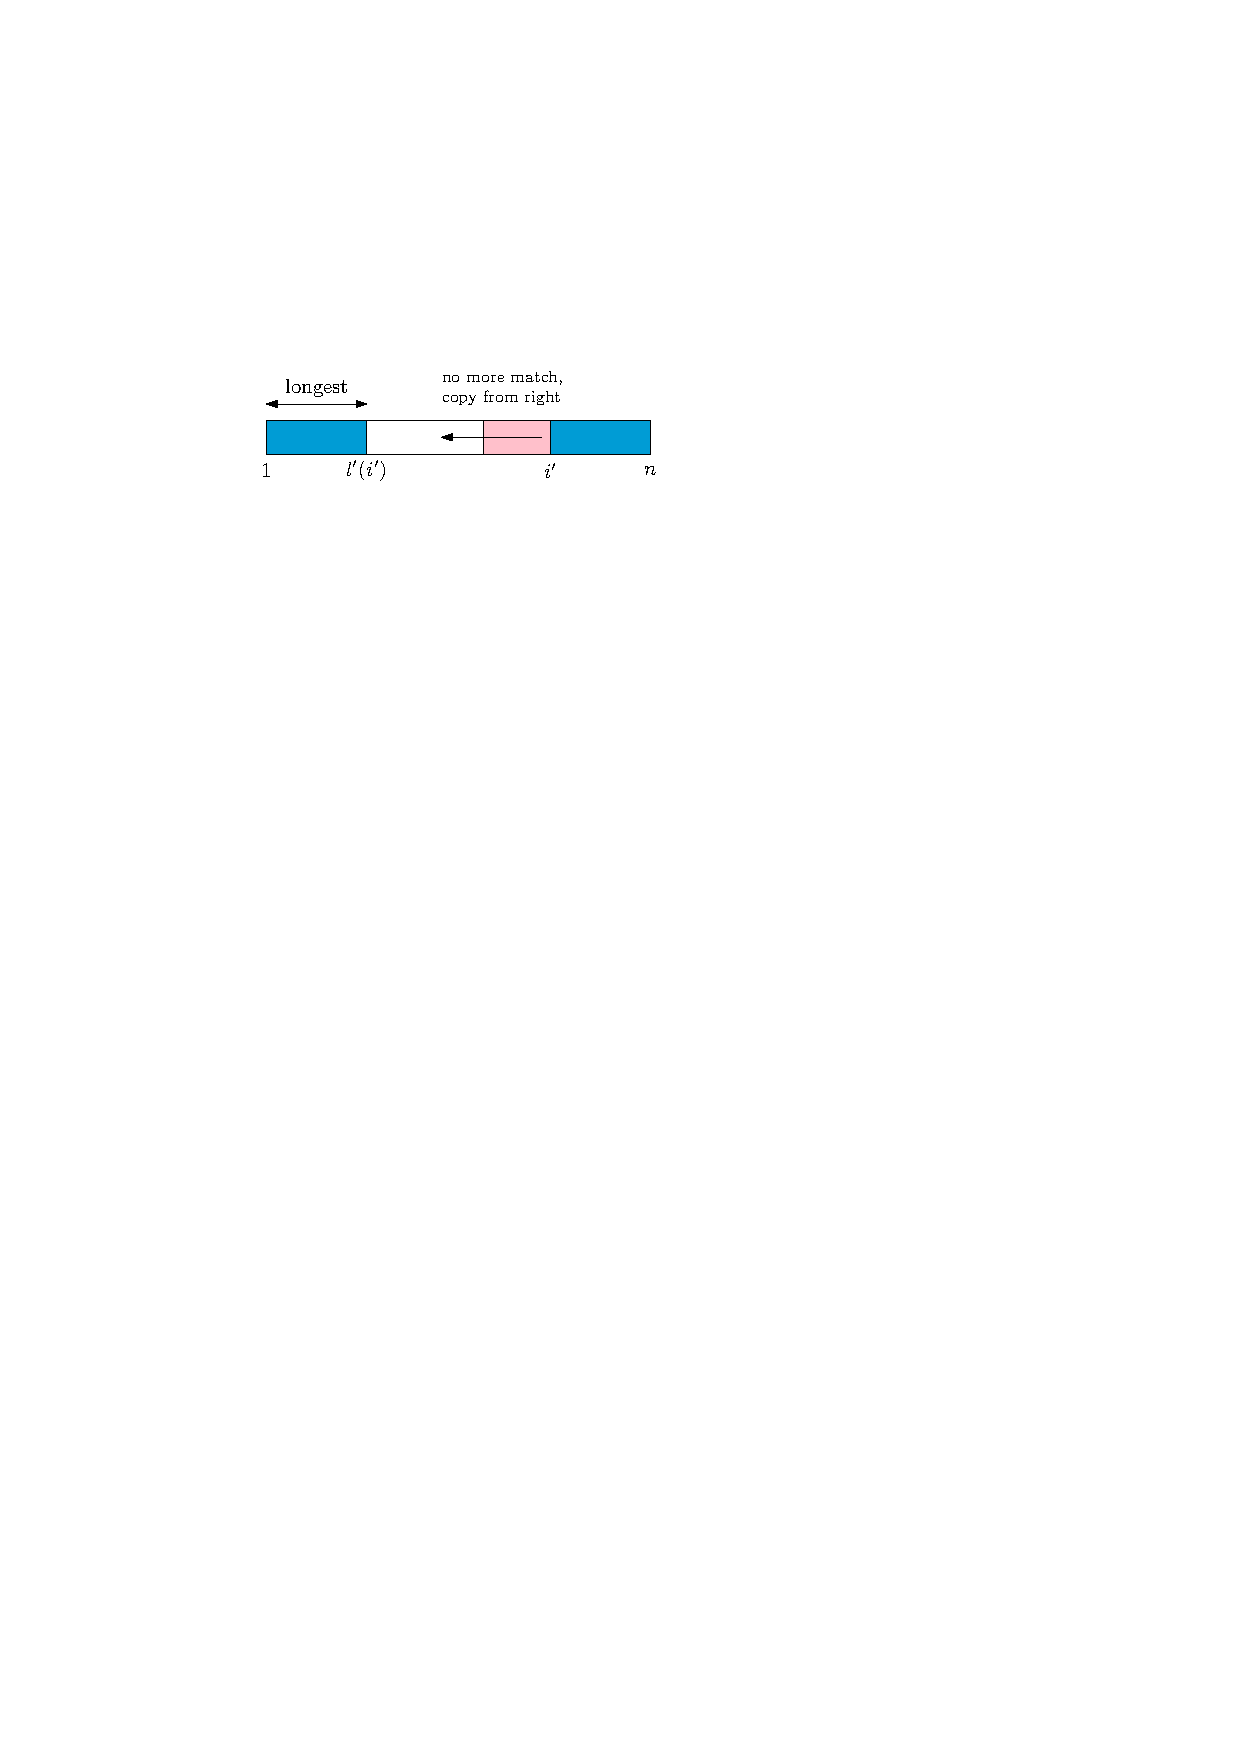
\includegraphics[width=\linewidth]{boyer-moore/good-suffix-ell-i-extension.pdf}
    \caption{``Smear'' to the left. This handles the cases when $P[i\ldots n]$ itself does not match a prefix of $P$, but some \textbf{proper suffix} $P[i' \ldots n]$ does.}
    \label{fig:good-suffix-ell-i-extension}
\end{marginfigure}
It copies the values of $l'$ from the right to fill in the blanks. Consider the example shown in Figure \ref{fig:good-suffix-ell-i-extension}. $P[1\ldots l'(i')]$ is the longest prefix that matches a suffix of $P$. For any $i < i'$, $P[i \ldots n]$ will not match a prefix of $P$. However, for those values of $i < i'$, $P[i'\ldots n]$ is \textbf{still a proper suffix} of $P[i \ldots n]$, so they ``inherit'' the $l'$ values from $l'(i')$ -- the left most position such that the entirety of $P[i'\ldots n]$ matches a prefix of $P$.

\section{Putting Everything Together}

\subsection{The Shifting Rules}

We summarize the shifting rules here. Remember that we are scanning from right to left.

\begin{enumerate}
    \item Bad character rule: Mismatch at $i$ with $T[k] \neq P[i]$; Shift $P$ to the right by $i - R(T[k])$.
    \item Good suffix rule: Mismatch at $i$ with $T[k] \neq P[i]$ but the suffix $P[i+1 \ldots n]$ matches some substring of $T$
    \begin{enumerate}
        \item If $L'(i) > 0$, then shift $P$ to the right by $n - L'(i)$
        \item If $L'(i) = 0$, then shift $P$ to the right by $n - l'(i)$ 
    \end{enumerate}
    \item No mismatch and $P$ is entirely matched with some substring of $T$, apply good suffix rule and shift $P$ to the right by $n - l'(2)$.
\end{enumerate}

\begin{figure}[htbp]
    \centering
    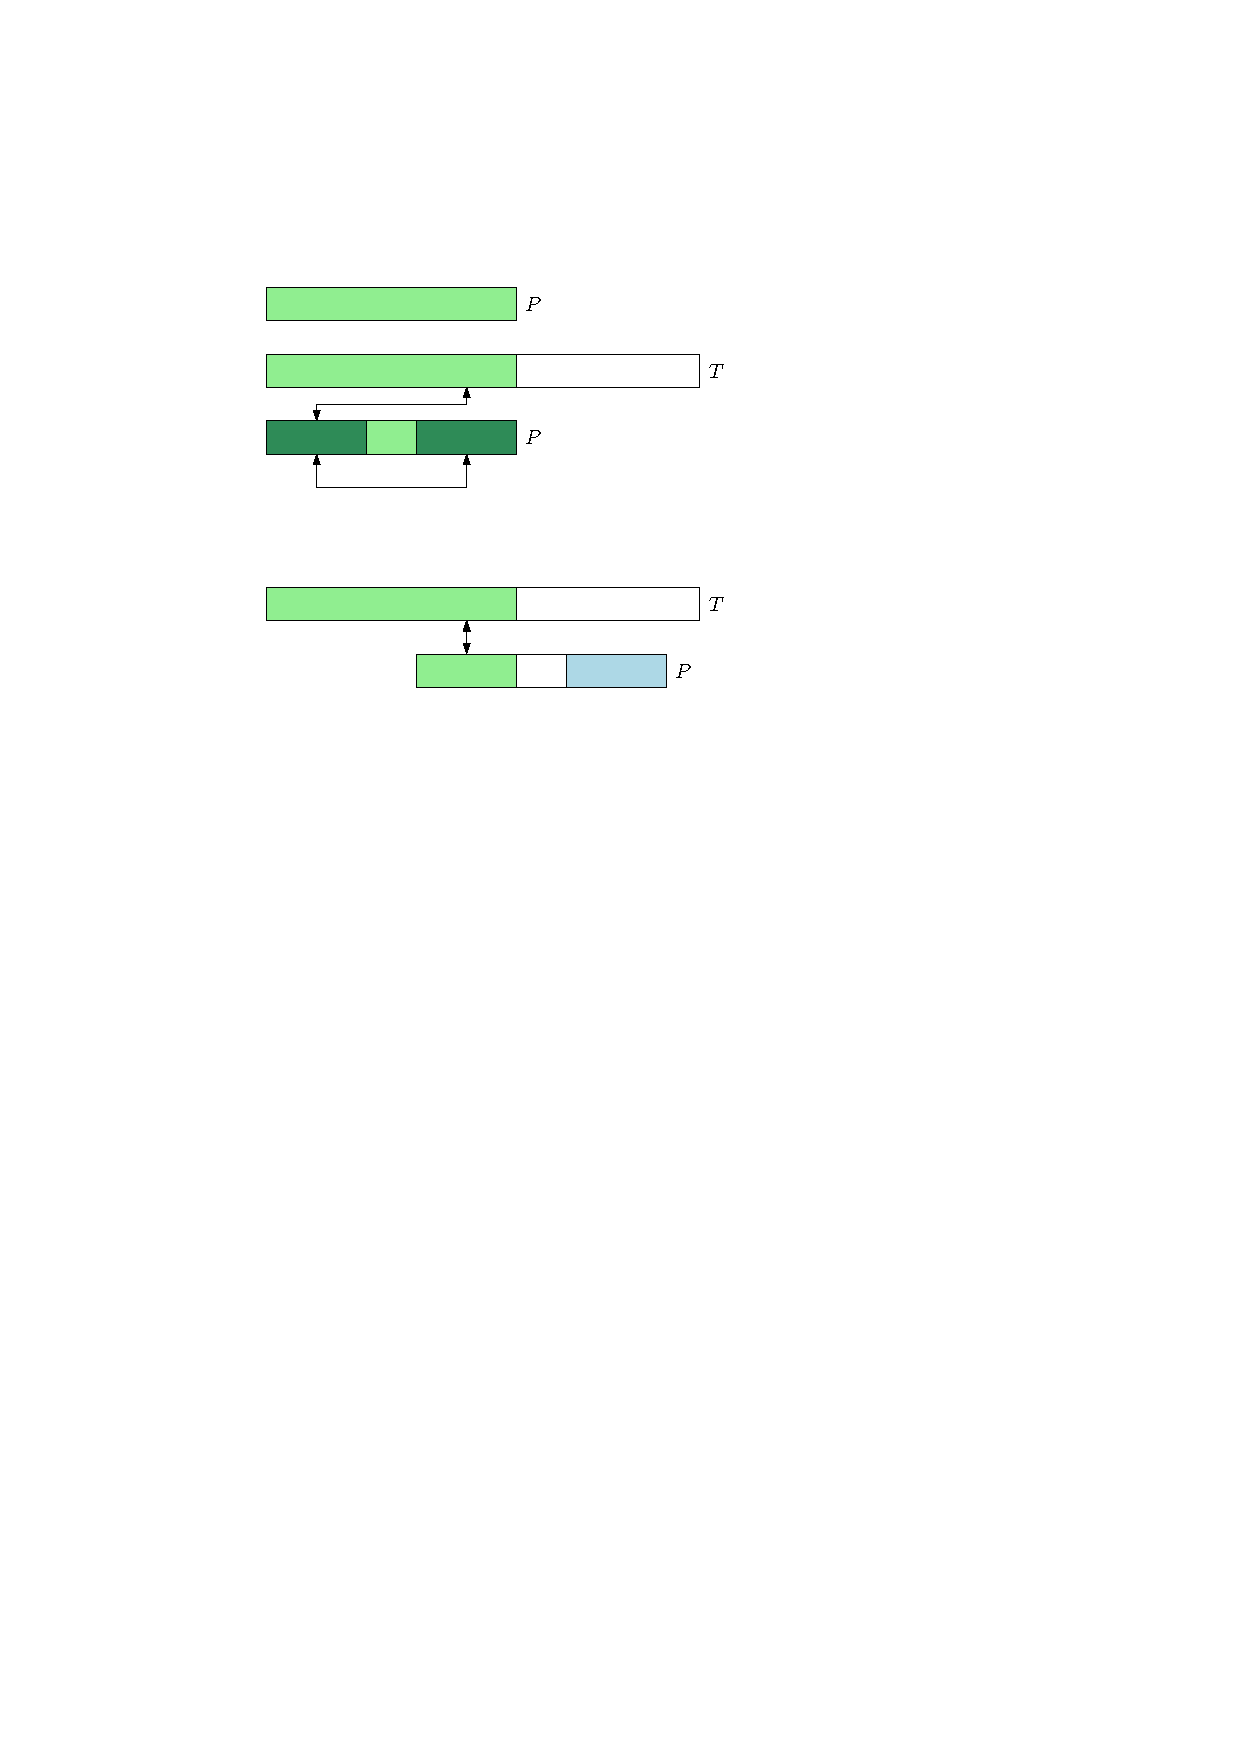
\includegraphics[width=0.6\linewidth]{boyer-moore/good-suffix-rule-full-match.pdf}
    \caption{The special good suffix rule when $P$ matches with $T$. We shift $P$ to the right so that a prefix of $P$ remains matched with $T$, if exists.}
    \label{fig:boyer-moore-good-suffix-rule-full-match}
\end{figure}

\subsection{Implementation}

For simplicity sake, we use $I$, the identity function when creating the bad character table. Again, in practice, if we are dealing with a sparse alphabet, we may want to change it to something else.

\begin{codebox}
    \Procname{$\proc{Boyer-Moore}(P,T)$}
    \li $L' = \proc{Compute-L'}(P)$
    \li $l' = \proc{Compute-$\ell'$}(P)$
    \li $R = \proc{Create-Bad-Character-Table}(P,I)$
    \li $k = |P|$
    \li \While $k \leq |T|$ \Do
        \li $i = n,\; h = k$
        \li \While $i > 0$ and $P[i] \isequal P[h]$ \Do
            \li $i = i - 1$
            \li $h = h - 1$
        \End
        \li \If $i = 0$ \Then
            \li $P$ found at position $h$ in $T$
            \li $k = k + |P| - l'[2]$
        \li \Else
            \li $\id{bc} = i - R[T[h]]$
            \li $\id{gs} = |P| - L'[i]$
            \li \If $\id{gs} \isequal 0$ \Then
                \li $\id{gs} = |P| - l'[i]$
            \End
            \li $k = k + \max\{\id{bc},\id{gs}\}$
\end{codebox}